\section{Noise}

\begin{frame}
  \frametitle{What is noise?}
  \begin{itemize}
  \item Models unpredictable behavior by adding a random variable.
  \item A random variable is a variable whose values are associated to a random phenomenon.
  \end{itemize}
\end{frame}

\section{Modeling}

\begin{frame}
  \frametitle{Modeling}
  \begin{columns}
  \column{0.5\textwidth} 
      \begin{itemize}
	\item Mathematical models are an abstraction of reality.
	\item There are three types of responses. 
	\begin{itemize}
		\item Type I\\
		$\ y'=\alpha y$
		\item Type II\\
		$\ y' = \frac{\alpha y}{y+ L}$ 
		\item Type III\\
		$\ y'= \frac {\alpha y^2}{\beta + y^2}$
	\end{itemize}
       \end{itemize}
  \column{0.5\textwidth}
      \begin {figure}
	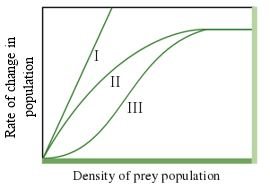
\includegraphics[scale = 0.7, right]{Responses}
       \end{figure}
  \end{columns}
\end{frame}

\begin{frame}
\frametitle{Modeling}
\begin{columns}[t]
\column{0.5\textwidth}
Deterministic Models
\begin{itemize}
\item Every set of variable states is determined by parameters in the model.
\item Always produce the same output from a given starting condition or initial state.
\end{itemize}

\column{0.5\textwidth}
Stochastic Models
\begin{itemize}
\item Variable states are not described by unique values, but rather by probability distributions.
\end{itemize}
\end{columns}

\bigskip
\centering
 Stochastic differential equations (SDEs) are systems described by differential equations influenced by random noise.
\end{frame}

\section{Random Walk}
\begin{frame}
  \frametitle{Random Walk}
  \begin{itemize}
  \item A random walk is a mathematical formalization of a path that consists of a succession of random steps.
  \end{itemize}
  \centering
  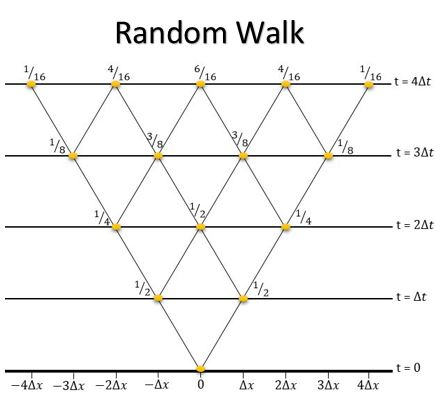
\includegraphics[scale=0.67]{RandomWalk}
\end{frame}

\begin{frame}
  \frametitle{Random Walk}
  \centering
%  \graphicspath{C:\Users\Valerie Ann\Documents\GitHub\REU15\Presentations\Midterm}
  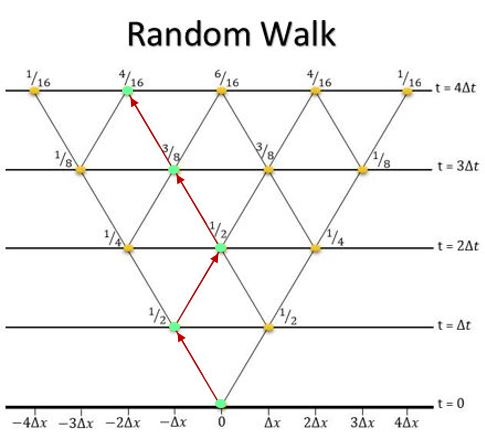
\includegraphics[scale=0.67]{RWPath}
\end{frame}